% Julian Burger
% Bastian Uhlig
% David Koch
% Gabriel Vogler

\documentclass[
	headings=optiontotocandhead,% Erweiterung für das optionale Argument der
	% Gliederungsbefehle aktiviert.
	oneside,
	numbers=noenddot,% Keine Punkte am Ende der Gliederungsnummern und davon
	% abgeleiteten Nummern
	toc=flat, %Flache TOC --- kann man anpassen (auskommentieren)
	10pt, % Schriftgröße
	parskip=full, % Abstand zwischen Absätzen (ganze Zeile)
	listof=totoc, % Verzeichnisse im Inhaltsverzeichnis aufführen
	listof=flat, % mehr Abstand für grosse Zahlen
	numbers=noenddot, % kein Punkt am Ende bei Nummern
	%%enlargefirstpage,% Gibt es bei scrartcl nicht!!!!
	bibliography=totoc, % Literaturverzeichnis im Inhaltsverzeichnis aufführen
	%index=totoc, % Index im Inhaltsverzeichnis aufführen
	%captions=tableheading, % Beschriftung von Tabellen für Ausgabe oberhalb
	% der Tabelle formatieren
	%draft % Status des Dokuments (final/draft) draft hinzufügen zum anziegen
	%%der zeilen ende
	a4paper,DIV=14,
	% captions=tablesignature,
]{scrartcl}
\usepackage{setspace}
\onehalfspacing

\setcounter{secnumdepth}{3}

\usepackage[usenames,dvipsnames,table]{xcolor} % Allows the definition and use of colors. This package has to be included before tikz.

\usepackage[T1]{fontenc}
\usepackage[utf8]{inputenc}

\usepackage[english, ngerman]{babel, varioref} % your native language must be the last one!!

\usepackage{lastpage}
\usepackage{listings}
\usepackage{blindtext}

\usepackage{tcolorbox}
\tcbuselibrary{skins}


%% Aufzählungen nicht so weit einrücken
\usepackage[inline]{enumitem}
%\setitemize{leftmargin=*}
% Listen etwas wenige einrücken, erfordert enumitem
\setitemize{labelindent=2em,labelsep=0.5cm,leftmargin=12ex}

\usepackage{lmodern}

\usepackage{xspace}

\usepackage{graphicx}
\graphicspath{ {.} } % Pfad(e) für Bilderimporte (es können mehrere angegeben werden, falls nötig)

%%? \usepackage{textcomp}
\usepackage[hyphens]{url}
\usepackage{makeidx}
\makeindex
%%? \usepackage{graphicx}
\usepackage[numbers]{natbib}
\PassOptionsToPackage{normalem}{ulem}
\usepackage{ulem}

\usepackage{needspace}

\setlength\partopsep{0.5ex}%schoenere Listen
\usepackage[bottom]{footmisc}%fussnote ganz unten

\usepackage[]{microtype}
\UseMicrotypeSet[protrusion]{basicmath} % disable protrusion for tt fonts

\usepackage{multirow}   % Allows table elements to span several rows.
\usepackage{booktabs}   % Improves the typesettings of tables.
\usepackage{subcaption} % Allows the use of subfigures and enables their referencing.
\usepackage[ruled,linesnumbered]{algorithm2e} % Enables the writing of pseudo code.
\usepackage{nag}       % Issues warnings when best practices in writing LaTeX documents are violated.
\usepackage{todonotes} % Provides tooltip-like todo notes.

\newcommand{\tabitem}{~~\llap{\textbullet}~~}

\usepackage{color}
\usepackage[binary-units]{siunitx}

%% Override default figure placement To be within the flow of the text rather
%% than on it's own page.
\usepackage{float}
\usepackage{placeins}
% \makeatletter
% \def\fps@figure{H}
% \makeatother

%% bei vielen Bildern o.ä sinnvoll: Seite muss nicht bis ganz unten gefüllt werden
% \raggedbottom

%\usepackage{footbib} %  footcite, needs other tooling
%% for pandoc2 images
\makeatletter
\def\maxwidth{\ifdim\Gin@nat@width>\linewidth\linewidth\else\Gin@nat@width\fi}
\def\maxheight{\ifdim\Gin@nat@height>\textheight\textheight\else\Gin@nat@height\fi}
\makeatother
% Scale images if necessary, so that they will not overflow the page
% margins by default, and it is still possible to overwrite the defaults
% using explicit options in \includegraphics[width, height, ...]{}
\setkeys{Gin}{width=\maxwidth,height=\maxheight,keepaspectratio}

%% bessere Suche im PDF
\input{glyphtounicode}
\pdfgentounicode=1
%%%%%%%%%%%%%%%%%%%%%%%%%%%%%%%%%%%%%%%%%%%%%%%%%%%%%%%%%%%%%%%%%%%%%%%%%%%%%%%%%%

%  Kopf und Fußzeilen -- links und rechts verschieden
\newcommand{\kopfTXT}{\sffamily{\textbf{\small{HÖHERE TECHNISCHE BUNDESLEHRANSTALT Wien 3 Rennweg}}\\
Höhere Abteilung für Mechantronik \\
Höhere Abteilung für Informationstechnologie\\
Fachschule für Informationstechnik}}

\tcbset{headerBoxStyle/.style={
          enhanced, frame hidden, interior hidden, top=-0.15cm, bottom=-0.1cm, borderline west = {4pt}{0pt}{red}
}}
\newtcolorbox{headerBox}[1][]{headerBoxStyle, #1}

\newcommand{\kopfbild}{\voffset7mm
\includegraphics[width=50mm]{HTL3RLogo}}
\newcommand{\kopfHTL}{\begin{headerBox}
\kopfTXT
\end{headerBox}}

\usepackage[automark,footsepline,plainfootsepline]{scrlayer-scrpage}
\setkomafont{pageheadfoot}{\normalcolor\footnotesize\scshape}
\setkomafont{pagenumber}{\normalfont\normalsize}
\clearpairofpagestyles
\ihead{\headmark}
\ohead{\kopfbild}
\ihead{\kopfHTL}
\ifoot{\smaller{DA Ansuchen}}
\ofoot{Seite \pagemark/\pageref{LastPage}}
\ModifyLayer[addvoffset=-.6ex]{scrheadings.foot.above.line}% Linie verschieben
\ModifyLayer[addvoffset=-.6ex]{plain.scrheadings.foot.above.line}% Linie verschieben
\setlength{\headheight}{46pt}

% alle Seiten mit Kopfzeile
%\renewcommand{\chapterpagestyle}{scrheadings}

%% Code Beispiele
%% eine Variante
\usepackage{listings}
\renewcommand{\lstlistingname}{\inputencoding{utf8}Listing}

\usepackage{tabularx}
\usepackage{tabularray}
\usepackage{scrhack}

\usepackage{array}
\newcommand\Tstrut{\rule{0pt}{3.2ex}}         % = `top' strut
\newcommand\Bstrut{\rule[-1.5ex]{0pt}{0pt}}   % = `bottom' strut

\newenvironment{nstabbing}
	{\setlength{\topsep}{-\parskip}
		\setlength{\partopsep}{-\parskip}
		\tabbing}
	{\endtabbing}

\usepackage{titlesec}
% \titleformat{?Überschriftenklasse?}[Absatzformatierung?]{?Textformatierung?} {?Nummerierung?}{?Abstand zwischen Nummerierung und Überschriftentext?}{?Code vor der Überschrift?}[?Code nach der Überschrift?]
\titleformat{\section}[hang]{\Large\bfseries\sffamily}{\thesection\quad}{-1.2ex}{}
\titleformat{\subsection}[hang]{\large\bfseries\sffamily}{\thesubsection\quad}{-1.2ex}{}
\titleformat{\subsubsection}[hang]{\large\bfseries\sffamily}{\thesubsubsection\quad}{-1.2ex}{}
\titleformat{\paragraph}[hang]{\large\bfseries\sffamily}{\theparagraph\quad}{-1.2ex}{}

% \titlespacing{?Überschriftenklasse?}{?Linker Einzug?}{?Platz oberhalb?}{?Platz unterhalb?}[?rechter Einzug?]
\titlespacing{\section}{0pt}{6pt}{6pt}
\titlespacing{\subsection}{0pt}{6pt}{0pt}
\titlespacing{\subsubsection}{0pt}{6pt}{0pt}
\titlespacing{\paragraph}{0pt}{6pt}{0pt}

%% sollte das letzte Package sein
\usepackage[unicode=true,
bookmarks=true,bookmarksnumbered=false,bookmarksopen=false,
breaklinks=true,pdfborder={0 0 0},backref=false,colorlinks=false]
{hyperref}
\hypersetup{pdftitle={Diplomarbeits-Ansuchen},
	pdfauthor={Wer auch immer},
	pdfsubject={DA},
	pdfkeywords={4xx, DA}}
\urlstyle{same} % don't use monospace font for urls

% Auch Fußnoten bündig ausrichten
\deffootnote[]{1em}{1em}{\textsuperscript{\thefootnotemark\ }}
%% setup
\sloppy % weniger Meldungen
\voffset7mm % etwas nach unten

\newcommand{\fieldbox}[4]{%
  \begin{tikzpicture}
    \draw[fill=white] (0,0) rectangle (#1,#2);
    \node[text=gray, font=\small] at (#1/2,0.2) {#3};
    \node[text=black, font=\large] at (#1/2,#2/1.5) {#4};
  \end{tikzpicture}%
}

\renewcommand{\familydefault}{\sfdefault} % Dokument sans serif
%\renewcommand\tabularxcolumn[1]{m{#1}}
%\renewcommand{\tabularxcolumn}[1]{>{\small}m{#1}}

%%%%%%%%%%%%%%%%%%%%%%%%%%%%%%%%%%%%%%%%%%%%%%%%%%%%%%%%%%%%%%%%%%%%%%%%%%%%%%%%%%
\begin{document}
%% schöner: 10000 -- gar keine, 1000 als Mittelweg
\clubpenalty = 10000 % Schusterjungen verhindern
\widowpenalty = 10000 % Hurenkinder verhindern
\displaywidowpenalty = 10000

{{\LARGE{{Ansuchen um Zulassung zur Diplomarbeit}}}}\\
\vspace{4mm}\\
\fieldbox{3.25cm}{1cm}{\footnotesize{Maturajahrgang}}{\large{2025}}
\hfill
\fieldbox{6cm}{1cm}{\footnotesize{Projektnummer (durch AV vergeben)}}{\large{}}\\ \\
\begin{tikzpicture}
  \draw[fill=white] (0,0) rectangle (\textwidth,1.68);
  \node[text=gray, font=\footnotesize, anchor=west] at (0.1,0.2) {Projektthema (Arbeitstitel)};
  \node[text=black, font=\Large, anchor=west] at (0.1,1.68/1.7) {\textbf{Titel der Diplomarbeit}};
\end{tikzpicture}


% Projektteam
\large{\textbf{Projektteam}}
\begin{table}[h]
\begin{tabularx} {\textwidth} {
	|>{\hsize=.364\hsize}X
	|>{\hsize=.094\hsize}X
	|>{\hsize=.173\hsize}X
	|>{\hsize=.369\hsize}X|
}

\hline
\rowcolor[HTML]{D9D9D9} 
\rule{0pt}{17pt}
\textbf{\normalsize{Schülerin/Schüler}} & \multicolumn{1}{c|}{\textbf{\normalsize{Klasse}}} & \multicolumn{1}{c|}{\textbf{\normalsize{\begin{tabular}[c]{@{}c@{}}Individuelle\\ Betreuung\end{tabular}}}} & \multicolumn{1}{c|}{\textbf{\normalsize{Unterschrift}}} \\ \hline
\rule{0pt}{28pt}	\large{\textbf{Vorname Nachname}}	&	\multicolumn{1}{c|}{\large{4XX}}	&	\multicolumn{1}{c|}{\large{KÜRZEL}}	&              \\

\rule{0pt}{11pt}\textcolor[HTML]{A6A6A6}{\footnotesize{Projektleiter:in}}	&	&	& \textcolor[HTML]{808080}{\footnotesize{Unterschrift Projektleiter:in}}	\\ \hline

\rule{0pt}{28pt}	\large{\textbf{Vorname Nachname}}	&	\multicolumn{1}{c|}{\large{4XX}}	&	\multicolumn{1}{c|}{\large{KÜRZEL}}	&              \\

\rule{0pt}{11pt}\textcolor[HTML]{A6A6A6}{\footnotesize{Stellv. Projektleiter:in}}	&	&	& \textcolor[HTML]{808080}{\footnotesize{Unterschrift Stellv. Projektleiter:in}}	\\ \hline

\rule{0pt}{28pt}	\large{\textbf{Vorname Nachname}}	&	\multicolumn{1}{c|}{\large{4XX}}	&	\multicolumn{1}{c|}{\large{KÜRZEL}}	&              \\

\rule{0pt}{11pt}\textcolor[HTML]{A6A6A6}{\footnotesize{Projektmitarbeiter:in}}		&	&	& \textcolor[HTML]{808080}{\footnotesize{Unterschrift Projektmitarbeiter:in}}	\\ \hline

\rule{0pt}{28pt}	\large{\textbf{Vorname Nachname}}	&	\multicolumn{1}{c|}{\large{4XX}}	&	\multicolumn{1}{c|}{\large{KÜRZEL}}	&              \\

\rule{0pt}{11pt}\textcolor[HTML]{A6A6A6}{\footnotesize{Projektmitarbeiter:in}}		&	&	& \textcolor[HTML]{808080}{\footnotesize{Unterschrift Projektmitarbeiter:in}}	\\ \hline
\end{tabularx}
\end{table}


\large{\textbf{Projektbetreuung:}}
\begin{table}[h]
\begin{tabularx} {\textwidth} {
	|>{\hsize=.462\hsize}X
	|>{\hsize=.538\hsize}X|
}

\hline
\rule{0pt}{28pt}	\large{\textbf{Vorname Nachname}}	&              \\
\rule{0pt}{11pt}\textcolor[HTML]{A6A6A6}{\footnotesize{Individuelle Betreuung (Hauptbetreuung)}}	&	\textcolor[HTML]{A6A6A6}{\footnotesize{Unterschrift Hauptbetreuer:in}}	\\ \hline
\rule{0pt}{28pt}	\large{\textbf{Vorname Nachname}}	&              \\
\rule{0pt}{11pt}\textcolor[HTML]{A6A6A6}{\footnotesize{Individuelle Betreuung (Hauptbetreuung Stellv.)}}	&	\textcolor[HTML]{A6A6A6}{\footnotesize{Unterschrift Stellv. Hauptbetreuer:iin}}	\\ \hline
\end{tabularx}
\end{table}


\large{\textbf{\textcolor[HTML]{A6A6A6}{Projektvergabe (durch AV):}}}

\begin{table}[h]
\begin{tabularx} {\textwidth} {
	|>{\hsize=.232\hsize}X
	|>{\hsize=.23\hsize}X
	|>{\hsize=.062\hsize}X
	|>{\hsize=.476\hsize}X|
}

\cline{1-2} \cline{4-4}
\rule{0pt}{17pt}\normalsize{\textcolor[HTML]{808080}{Hauptbetreuung:}}&&&\\ \cline{1-2}
\rule{0pt}{17pt}\normalsize{\textcolor[HTML]{808080}{HB Stellvertretung:}}&&&\\ \cline{1-2}
\rule{0pt}{17pt}\normalsize{\textcolor[HTML]{808080}{Indiv. Betreuungen:}}&&&\footnotesize{\textcolor[HTML]{808080}{Bewilligt (Unterschrift AV)}}\\ \cline{1-2} \cline{4-4}
\end{tabularx}
\end{table}

\newpage

\tableofcontents
\newpage

\section{Projektidee}

\subsection{Ausgangssituation}
Kurze Beschreibung der Voraussetzungen und Rahmenbedingungen des Projekts (Wie ist es zu dem Projekt gekommen, welche Rand- und Rahmenbedingungen gibt es?). Diese Anmerkung und alle anderen in dem Text (hellgraue Absätze wie dieser hier) bitte löschen, bevor das Dokument abgegeben wird. 

Lorem ipsum dolor sit amet, consetetur sadipscing elitr, sed diam nonumy eirmod tempor invidunt ut labore et dolore magna aliquyam erat, sed diam voluptua. At vero eos et accusam et justo duo dolores et ea rebum. 

Stet clita kasd gubergren, no sea takimata sanctus est Lorem ipsum dolor sit amet. Lorem ipsum dolor sit amet, consetetur sadipscing elitr, sed diam nonumy eirmod tempor invidunt ut labore et dolore magna aliquyam erat, sed diam voluptua. At vero eos et accusam et justo duo dolores et ea rebum. Stet clita kasd gubergren, no sea takimata sanctus est Lorem ipsum dolor sit amet.

\subsection{Beschreibung der Idee}
Kurze Beschreibung der Projektidee, eventuell mit Skizzen, Schemata oder Grafiken

Lorem ipsum dolor sit amet, consetetur sadipscing elitr, sed diam nonumy eirmod tempor invidunt ut labore et dolore magna aliquyam erat, sed diam voluptua. At vero eos et accusam et justo duo dolores et ea rebum. 

Stet clita kasd gubergren, no sea takimata sanctus est Lorem ipsum dolor sit amet. Lorem ipsum dolor sit amet, consetetur sadipscing elitr, sed diam nonumy eirmod tempor invidunt ut labore et dolore magna aliquyam erat, sed diam voluptua. At vero eos et accusam et justo duo dolores et ea rebum. Stet clita kasd gubergren, no sea takimata sanctus est Lorem ipsum dolor sit amet.

\newpage

\newpage
\section{Projektziele}
\subsection{Hauptziele}
Auflistung der einzelnen Ziele als Zustand, Beschreibung inklusive Lösungsansatz. Soweit wie möglich granular heruntergebrochen als einzelne Anforderung. Wenn gemeinsam an einem Ziel gearbeitet wird, ist das Ziel in Sub-Ziele aufzusplitten, so dass ein Subziel nur einem/einer Schüler:in zugeordnet ist (siehe Ziel H2a und Ziel H2b). Alle Ziele müssen SMART definiert sein.
 
\begin{enumerate}[start=1,label={\bfseries Ziel-H \arabic*},leftmargin=*,wide]
\item{\bfseries{Lorem Ipsum}}\\
Lorem Ipsum, lorem ipsum, lorem ipsum, lorem ipsum, lorem ipsum, lorem ipsum, lorem ipsum, lorem ipsum, lorem ipsum

\item{\bfseries{Online Zahlungsmethode}}\\
Eine Online Zahlungsmethode ist im Bestellvorgang des Online Shops implementiert.

\begin{enumerate}[label=\alph*.]
\item{Online Zahlungsmethoden werden analysiert und bewertet. Nach Bewertung der Kompatibilität wird eine für den User geeignete und sichere Methode als Zahlungsvariante in den Bestellvorgang gewählt.}\\

\item{Das Zahlungssytem wird in einem Testsystem eingebunden. Nach erfolgreichen Tests wird die Bezahlmethode im Produktivsystem implementiert.}\\
\end{enumerate}

\item{\bfseries{Dummy}}\\
\end{enumerate}

\subsection{Optionale Ziele}
Auflistung der einzelnen Ziele als Zustand, Beschreibung inklusive Lösungsansatz. Alle Ziele müssen SMART definiert sein.

\begin{enumerate}[start=1,label={\bfseries Ziel-O \arabic*},leftmargin=*,wide]
\item{\bfseries{Dummy}}\\
Lorem Ipsum, lorem ipsum, lorem ipsum, lorem ipsum, lorem ipsum, lorem ipsum, lorem ipsum, lorem ipsum, lorem ipsum
\end{enumerate}

\subsection{NICHT Ziele}
Achtung, NICHT ZIELE werden positiv formuliert und sollen das Projekt eingrenzen. Dienen vor allem auch zur Sicherheit des Projektleiters, da explizit formuliert wird, was NICHT geliefert wird.

\begin{enumerate}[start=1,label={\bfseries Ziel-N \arabic*},leftmargin=*,wide]
\item{\bfseries{Dummy}}\\
Lorem Ipsum, lorem ipsum, lorem ipsum, lorem ipsum, lorem ipsum, lorem ipsum, lorem ipsum, lorem ipsum, lorem ipsum
\end{enumerate}
\newpage

\subsection{Individuelle Aufgabenstellungen der Teammitglieder im Projekt}
Jedes Ziel aus 2.1. und 2.2. oder ein spezifischer Teil davon muss genau einem Teammitglied zugeordnet werden. Ein Ziel kann also nicht bei mehreren Teammitgliedern stehen. Diese Person ist für die Erfüllung dieses Zieles verantwortlich und wird zu diesen Inhalten auch in der Defensio befragt. Das heißt nicht, dass man sich im Team nicht aushelfen darf.

\begin{table}[H]
	\begin{tabularx} {\textwidth} {
			|>{\hsize=1\hsize}X|
		}
		
		\hline
		\rowcolor[HTML]{D9D9D9} 
		\rule{0pt}{15pt}
		\textbf{\normalsize{Vorname Nachname - Projektleiter:in}} \\ \hline
		
		\rule{0pt}{20pt} \\
		\rule{0pt}{11pt}\textcolor[HTML]{A6A6A6}{\footnotesize{Themenschwerpunkt: Kurze Beschreibung des Themenschwerpunkts in ein paar Sätzen}} \\ \hline
		
		\begin{itemize}[itemsep=0pt, parsep=0pt, topsep=0pt]
			\item{ZIEL-H 2a Online Zahlungsmethode – Analyse und Bewertung}
			\item{ZIEL-H 4a Dummy}
			\item{ZIEL-H X Dummy}
			\item{ZIEL-O 1a Dummy}
		\end{itemize}
		
		\rule{0pt}{11pt}\textcolor[HTML]{A6A6A6}{\footnotesize{Aufgabenstellung: Auflistung der einzelnen Ziele und Anforderungen}} \\ \hline
	\end{tabularx}
\end{table}

\begin{table}[H]
	\begin{tabularx} {\textwidth} {
			|>{\hsize=1\hsize}X|
		}
		
		\hline
		\rowcolor[HTML]{D9D9D9} 
		\rule{0pt}{15pt}
		\textbf{\normalsize{Vorname Nachname - Rolle Mitarbeiter:in}} \\ \hline
		
		\rule{0pt}{20pt} \\
		\rule{0pt}{11pt}\textcolor[HTML]{A6A6A6}{\footnotesize{Themenschwerpunkt: Kurze Beschreibung des Themenschwerpunkts in ein paar Sätzen}} \\ \hline
		
		\begin{itemize}[itemsep=0pt, parsep=0pt, topsep=0pt]
			\item{ZIEL-H 2b Online Zahlungsmethode – Implementierung}
			\item{ZIEL-H Y Dummy}
			\item{ZIEL-O 1b Dummy}
			\item{ZIEL-O X Dummy}
		\end{itemize}
		
		\rule{0pt}{11pt}\textcolor[HTML]{A6A6A6}{\footnotesize{Aufgabenstellung: Auflistung der einzelnen Ziele und Anforderungen}} \\ \hline
	\end{tabularx}
\end{table}

\begin{table}[H]
	\begin{tabularx} {\textwidth} {
			|>{\hsize=1\hsize}X|
		}
		
		\hline
		\rowcolor[HTML]{D9D9D9} 
		\rule{0pt}{15pt}
		\textbf{\normalsize{Vorname Nachname - Rolle Mitarbeiter:in}} \\ \hline
		
		\rule{0pt}{20pt} \\
		\rule{0pt}{11pt}\textcolor[HTML]{A6A6A6}{\footnotesize{Themenschwerpunkt: Kurze Beschreibung des Themenschwerpunkts in ein paar Sätzen}} \\ \hline
		
		\begin{itemize}[itemsep=0pt, parsep=0pt, topsep=0pt]
			\item{ZIEL-H 1 Dummy}
			\item{ZIEL-H 3 Dummy}
			\item{ZIEL-H Z Dummy}
			\item{ZIEL-O 1c Dummy}
		\end{itemize}
		
		\rule{0pt}{11pt}\textcolor[HTML]{A6A6A6}{\footnotesize{Aufgabenstellung: Auflistung der einzelnen Ziele und Anforderungen}} \\ \hline
	\end{tabularx}
\end{table}

\newpage
\section{Projektorganisation}
\subsection{Grafische Darstellung}

\begin{figure}[h]
	\centering
	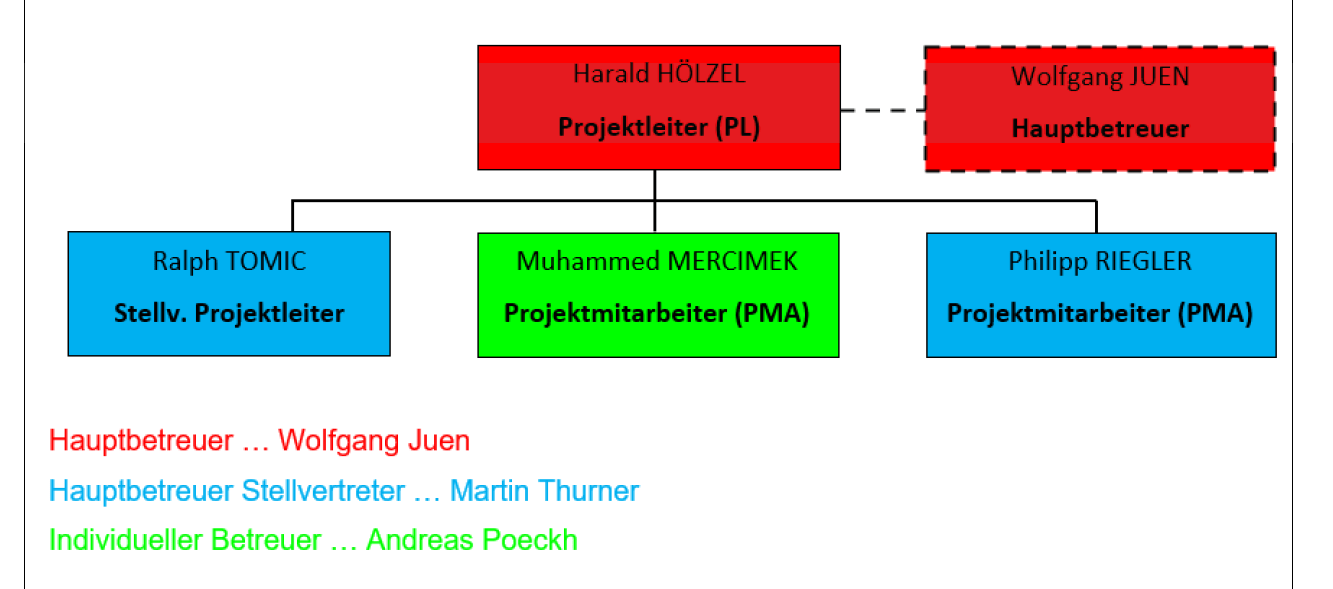
\includegraphics[width=1\linewidth]{Organigramm_1}
	\caption[]{Erstes Beispiel eines Projektorganigramms}
\end{figure}
\FloatBarrier 

\begin{figure}[h]
	\centering
	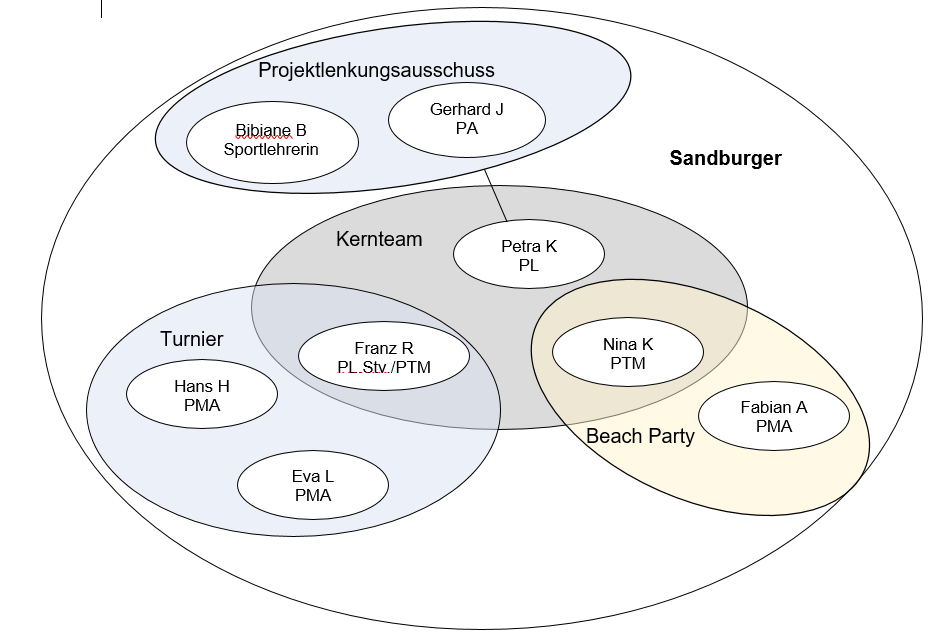
\includegraphics[width=1\linewidth]{Organigramm_2}
	\caption[]{Zweites Beispiel eines Projektorganigramms}
\end{figure}
\FloatBarrier 

{\small\begin{spacing}{1.125}
Legende: \\
PA = Projektauftraggeber \\
PL = Projektleiter \\
PL-Stv = Projektleiter Stellvertretung \\
PMA = Projektmitarbeiter \\
H-Betreuung = Hauptbetreuung \\
Betreuung-Stv = Betreuung Stellvertretung \\
\end{spacing}}

\subsection{Projektteam}
\begin{table}[h]
	\begin{tabularx} {\textwidth} {
			|>{\hsize=.12\hsize}c
			|>{\hsize=.38\hsize}X
			|>{\hsize=.09\hsize}c
			|>{\hsize=.41\hsize}X|
		}
		
		\hline
		\rowcolor[HTML]{D9D9D9} 
		\rule{0pt}{17pt}
		\textbf{\normalsize{Funktion}} & {\textbf{\normalsize{Name}}} & {\textbf{\normalsize{Kürzel}}} & {\textbf{\normalsize{E-Mail}}} \\ \hline
		\rule{0pt}{15pt}	PL & & & \\ \hline
		\rule{0pt}{15pt}	PL Stv. & & & \\ \hline
		\rule{0pt}{15pt}	PMA & & & \\ \hline
		\rule{0pt}{15pt}	PMA & & & \\ \hline
	\end{tabularx}
\end{table}

\newpage
\section{Betrachtungsplan}

\begin{figure}[h]
	\centering
	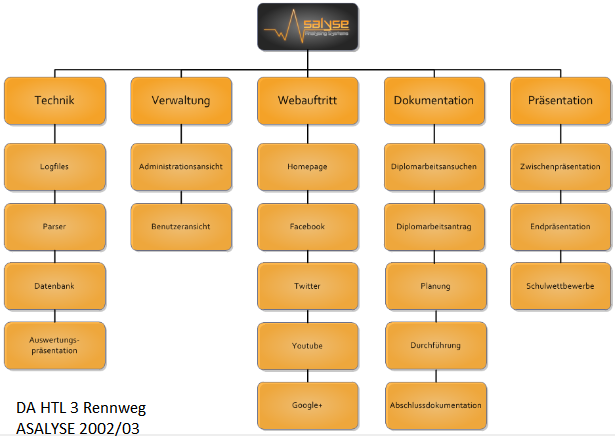
\includegraphics[width=1\linewidth]{OSP_1}
	\caption[]{Erstes Beispiel für ein Betrachtungsplan}
\end{figure}
\FloatBarrier 
oder
\begin{figure}[h]
	\centering
	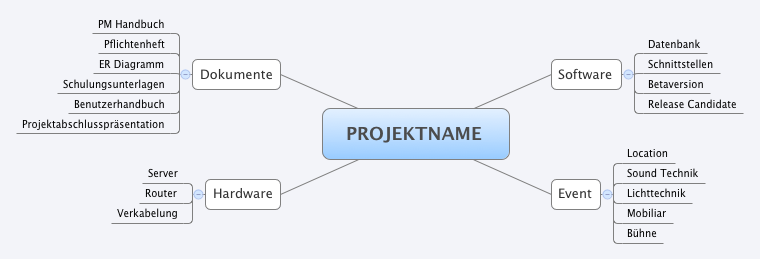
\includegraphics[width=1\linewidth]{OSP_2}
	\caption[]{Zweites Beispiel für ein Betrachtungsplan}
\end{figure}
\FloatBarrier 

\newpage
\section{Budget}
\subsection{Erwartete Kosten für die Durchführung des Projektes}
\begin{table}[h]
	\begin{tabularx} {\textwidth} {
			|>{\hsize=.07\hsize}X
			|>{\hsize=.8\hsize}X
			|>{\hsize=.13\hsize}X|
		}
		
		\hline
		\rowcolor[HTML]{D9D9D9} 
		\rule{0pt}{17pt}
		\textbf{\normalsize{Pos}} & {\textbf{\normalsize{Bezeichnung des Aufwands}}} & \multicolumn{1}{r|}{\textbf{\normalsize{Kosten}}} \\ \hline
		\rule{0pt}{15pt}	1 & Einmalige Setupgebühr Payment-Provider & \multicolumn{1}{r|}{€ 300} \\ \hline
		\rule{0pt}{15pt}	2 & Serverkosten für 1 Jahr & \multicolumn{1}{r|}{€ 120} \\ \hline
		\rule{0pt}{15pt}	3 & Druckkosten für 500 Flyer & \multicolumn{1}{r|}{€ 40} \\ \hline
		\rowcolor[HTML]{D9D9D9} 
		\rule{0pt}{15pt}
		 & {\normalsize{Gesamtkosten}} & \multicolumn{1}{r|}{\normalsize{€ 460}} \\ \hline
	\end{tabularx}
\end{table}

\subsection{Kostendeckung}
Kurze Beschreibung, wie die Kosten gedeckt werden. Die Finanzierung muss vor Projektstart geklärt sein.

Lorem ipsum dolor sit amet, consetetur sadipscing elitr, sed diam nonumy eirmod tempor invidunt ut labore et dolore magna aliquyam erat, sed diam voluptua. At vero eos et accusam et justo duo dolores et ea rebum. 

Stet clita kasd gubergren, no sea takimata sanctus est Lorem ipsum dolor sit amet. Lorem ipsum dolor sit amet, consetetur sadipscing elitr, sed diam nonumy eirmod tempor invidunt ut labore et dolore magna aliquyam erat, sed diam voluptua. At vero eos et accusam et justo duo dolores et ea rebum. Stet clita kasd gubergren, no sea takimata sanctus est Lorem ipsum dolor sit amet.

\newpage
\section{Geplante externe Kooperationspartner}
Auflistung der geplanten externen Kooperationspartner. Diese müssen im Antrag dann bereits fixiert sein.\\
Es muss die Art der Kooperation angeführt werden (Firma als Auftraggeber, Beratung durch die Firma im Bereich XY, Fertigung von Teilen des Projekts durch das Unternehmen, Sponsoring und Präsentation des Projektes im Unternehmen, etc.).\\
Nur der reine Kauf von Bauteilen oder einer speziellen Software bei einem Unternehmen ist keine Kooperation.

Lorem ipsum dolor sit amet, consetetur sadipscing elitr, sed diam nonumy eirmod tempor invidunt ut labore et dolore magna aliquyam erat, sed diam voluptua. At vero eos et accusam et justo duo dolores et ea rebum. 
\begin{itemize}
	\item{Kooperationspartner 1}
	\item{Kooperationspartner 2}
\end{itemize}
Stet clita kasd gubergren, no sea takimata sanctus est Lorem ipsum dolor sit amet. Lorem ipsum dolor sit amet, consetetur sadipscing elitr, sed diam nonumy eirmod tempor invidunt ut labore et dolore magna aliquyam erat, sed diam voluptua. At vero eos et accusam et justo duo dolores et ea rebum. Stet clita kasd gubergren, no sea takimata sanctus est Lorem ipsum dolor sit amet.

\newpage
\section{Geplante Verwertung der Ergebnisse}
Kurze Beschreibung, wie das Ergebnis der Diplomarbeit verwertet, weiterverwendet werden soll bzw. was mit dem Ergebnis nach Abschluss der Arbeit passiert (d.h. was passiert am Ende des Projektes mit dem Produkt? An wen wird es wann übergeben? Wer nimmt es ev. mit nach Hause?).

Lorem ipsum dolor sit amet, consetetur sadipscing elitr, sed diam nonumy eirmod tempor invidunt ut labore et dolore magna aliquyam erat, sed diam voluptua. At vero eos et accusam et justo duo dolores et ea rebum. 

Stet clita kasd gubergren, no sea takimata sanctus est Lorem ipsum dolor sit amet. Lorem ipsum dolor sit amet, consetetur sadipscing elitr, sed diam nonumy eirmod tempor invidunt ut labore et dolore magna aliquyam erat, sed diam voluptua. At vero eos et accusam et justo duo dolores et ea rebum. Stet clita kasd gubergren, no sea takimata sanctus est Lorem ipsum dolor sit amet.

\end{document}
